\documentclass[fleqn]{scrartcl}
\usepackage{amsmath}
\usepackage{amsfonts}
\usepackage{amssymb}
\usepackage{enumerate}
%% Support for the target language %%%%%%%%%%%%%%%%%%%%%%%%%%%%%%%%%%%%
\usepackage[ngerman]{babel}

%% Font & encoding %%%%%%%%%%%%%%%%%%%%%%%%%%%%%%%%%%%%%%%%%%%%%%%%%%%%
\usepackage[T1]{fontenc}
\usepackage[utf8]{inputenc}

%% Custom headings %%%%%%%%%%%%%%%%%%%%%%%%%%%%%%%%%%%%%%%%%%%%%%%%%%%%
\usepackage[explicit]{titlesec}

%% Shows the use of deprecated stuff %%%%%%%%%%%%%%%%%%%%%%%%%%%%%%%%%%
\usepackage{nag}

%% Code listings %%%%%%%%%%%%%%%%%%%%%%%%%%%%%%%%%%%%%%%%%%%%%%%%%%%%%%
\usepackage{listings}

%% Advanced math %%%%%%%%%%%%%%%%%%%%%%%%%%%%%%%%%%%%%%%%%%%%%%%%%%%%%%
\usepackage{amsmath}

%% Advanced math Symboles %%%%%%%%%%%%%%%%%%%%%%%%%%%%%%%%%%%%%%%%%%%%%
\usepackage{amssymb}

%% Introducing proof environments %%%%%%%%%%%%%%%%%%%%%%%%%%%%%%%%%%%%%
\usepackage{amsthm}

%% Just the \lightning symbol %%%%%%%%%%%%%%%%%%%%%%%%%%%%%%%%%%%%%%%%%
\usepackage{stmaryrd}

%% For commutative diagrams %%%%%%%%%%%%%%%%%%%%%%%%%%%%%%%%%%%%%%%%%%%
\usepackage[all]{xy}

%% Table with extended features %%%%%%%%%%%%%%%%%%%%%%%%%%%%%%%%%%%%%%%
\usepackage{tabularx}

%% Graphic handling %%%%%%%%%%%%%%%%%%%%%%%%%%%%%%%%%%%%%%%%%%%%%%%%%%%
\usepackage{graphicx}

%% Table coloring %%%%%%%%%%%%%%%%%%%%%%%%%%%%%%%%%%%%%%%%%%%%%%%%%%%%%
\usepackage[table]{xcolor}

\usepackage{setspace}

%% Formatting %%%%%%%%%%%%%%%%%%%%%%%%%%%%%%%%%%%%%%%%%%%%%%%%%%%%%%%%%

\renewcommand{\labelitemii}{$\bullet$}

\setlength\parindent{0pt}

\newcommand{\qq}[1]{\glqq #1\grqq}

\newcommand{\q}[1]{\glq #1\grq}

\newcommand{\definition}[1]{\glq #1\grq}

\renewenvironment{proof}{{\bfseries Beweis }}{\qed}

\newenvironment{example}{{\bfseries Beispiel }}{}

\newtheorem{theorem}{Satz}

\begin{document}
\title{Analysis I Skript}
\date{9.11.2013}
\author{Rene Brandel und Rudolf Biczok}
\maketitle
\section{Grundlagen}

\subsection{Mengen}

Angaben von Mengen durch Aufzählungen

$M=\left\{ a,b,c \right\}$ oder $M=\left\{ Kirche, Dorf\right\}$

bekannte Mengen:
\begin{itemize}
  \item $\emptyset$ leere Menge
  \item $\mathbb{N} = \left\{ 1,2,3,\ldots \right\}$ natürliche Zahlen
  \item $\mathbb{Z} = \left\{ \ldots,-3,-2,-1,0,1,2,3,\ldots \right\}$ ganze Zahlen
  \item $\mathbb{Q} = \left\{ \frac{m}{n}|m \in \mathbb{Z},n \in \mathbb{N} \right\}$ Rationale Zahlen
\end{itemize}

\textbf{Achtung:} $\left\{ \emptyset \right\}$ hat ein Element (nämlich die leere Menge)!

\subsubsection{Syntax}

\begin{itemize}
  \item $x \in M$ $x$ ist Element von $M$
  \item $x \notin M$ $x$ ist nicht Element von $M$
  \item $M \subset N$ $M$ ist Teilmenge von $N$
  d.h. für alle $x \in M$ ist auch $x \in N$ \\
  \textbf{Achtung:} Bei $M \subset N $ ist auch $M = N$ möglich \\
  \textbf{Immer:} $\emptyset \subset M$,in jeder Menge
  \item $M=N: M \subset N \wedge N \subset N$
  \item Vereinigungsmenge: $M \cup N := \left\{ x|x \in M \wedge x \in N\right\}$
  \item Disjunktion: $M$ und $N$ sind disjunkt wenn $M  \cup N = \emptyset$ 
  \item Schnittmenge: $M \cap N := \left\{ x|x \in M \vee x \in N\right\}$ 
  \item Differenz: $M \backslash N := \left\{ x|x \in M \wedge x \notin N \right\}$ 
  \item Produktmenge: $M \times N:= \left\{ (x,y)|x \in M, y \in N \right\}$  \\
  $M_1 \times M_2 \times \ldots \times M_n := \{ \underbrace{(x_1,x_2,\ldots,x_n)}_{\text{n-Tupel}} : x_j \in M_j, j= 1,\ldots,n \}$
\end{itemize}

\subsubsection{Satz 1: \qq{Naiver} Mengenbegriff nach Cantor}

\qq{Unter einer \q{Menge} verstehen wir jede Zusammenfassung M von bestimmten wohlunterschiedenen Objekten m unserer Anschauung oder unseres Denkens (welche die \q{Elemente} von M genannt werden) zu einem Ganzen.}

\subsubsection{Potenzmenge von M}

$2^M = \mathcal{P}(M) := \left\{ A | A \subset M \right\}$

\textbf{immer:} $ M \in \mathcal{P}(M), \emptyset \in \mathcal{P}(M)$ 

\begin{example}{$\mathcal{P}(\emptyset) = \left\{ \emptyset \right\}$}
\end{example}

\subsubsection{Satz 2: Funktionen}

Eine Funktion oder Abbildung $f : x \to y$ besteht aus einem Definitionsbereich $X$ und einer Abbildungsvorschrift, die jedem $x \in X$ genau ein Element $y \in Y$ zuordnet.

\textbf{Notation} $y=f(x)$, erfordert auf $x \mapsto f(x)$
\begin{align*}
  f : X &\to Y\\
  x &\mapsto f(x)
\end{align*}

\begin{example}
\begin{align*}
  f : \mathbb{N} &\to \mathbb{N}\\
  x &\mapsto f(x) = 2x
\end{align*}
\end{example}

\subsubsection{Satz 3: Graph}

Sei $f:X \to Y$ eine Funktion

$Graph(f) = G(f) = \left\{ (x,f(x)) : x \in X \right\}$

$G(f) \subset X \times Y$

Zwei Funktionen $f_1 : X \to Y, f_2 : X \to Y$ sind gleich, wenn $G(f_1) = G(f_2)$. D.h. falls $f_1(x)=f_2(x)$ für alle $x \in X$.

\subsubsection{Funktionsraum}

$Y^X = Abb(X,Y) = $ Menge aller Funktionen $f : X \to Y$

\subsubsection{Bild}

Wenn $A \subset X$:

$f(A):=\left\{ y \in Y : \text{ Es gibt ein } x \in A : y=f(x) 
\right\} =\left\{ f(x) : x \in A \right\}$

Bild von $A$ (unter $f$)

\subsubsection{Urbild}

Wenn $B \subset Y$ 

$f^{-1}(B):=\left\{ x \in X : f(x) \in B \right\}$

Urbild von $B$ (unter $f$)

\subsubsection{Eigenschaften von Funktionen}

$f(X)$ ist das Bild von $f$

$f : X \to Y$ ist:

\begin{description}
\item[injektiv:] falls aus $x_1,x_2 \in X$ und $f(x_1)=f(x_2) \implies x_1=x_2$. 

\item[surjektiv:] falls $f(X) = Y$.

\item[bijektiv:] falls surjektiv und injektiv zugleich.
\end{description}

\subsubsection{Umkehrabbildung / Umkehrfunktion}

Ist $f : X \to Y$ bijektiv, so existiert zu jedem $y \in Y$ genau ein $x \in X$ mit $y =f(x)$. Die Inverse zu $f$ ist die Funktion: 
\begin{align*}
  f^{-1} : Y &\to X\\
  y &\mapsto \text{ Urbild von } Y \text{ unter } f
\end{align*}

\begin{example}
\begin{align*}
  f : \mathbb{N} & \to     \mathbb{N}\\
                    x & \mapsto 2x
\end{align*}
$ f^{-1}(\{3\}) = \emptyset $

$\rightarrow$ ist nicht bijektiv

\[P : N \to \text{gerade natürliche Zahlen}\]
\begin{align*}
  f : P(\mathbb{N}) & \to     P(\mathbb{N})\\
                       x & \mapsto 2x
\end{align*}
\end{example}

$\rightarrow$ ist bijektiv

$f^{-1}(y)=\frac{y}{2} \in \mathbb{N},y=$ gerade natürliche Zahl.

\subsubsection{Komposition}

Sei $f : X \to Y, g : W \to Z$ mit $f(X) \subset W$

$h:= g \circ f$ ($g$ ist verknüpft mit $f$)
$h(x):= (g \circ f)(x):=g(f(x))$

\subsubsection{Identität}

\begin{align*}
  id_M : M & \to     M\\
              x & \mapsto x
\end{align*}

Sei: $f : M \to N$ bijektiv, dann gilt:

\begin{enumerate}
 \item $f^{-1} : N \to M \text{ existiert} $
 \item $f^{-1} \circ f = id_M$
 \item $f \circ f^{-1} = id_N$
\end{enumerate}

\subsubsection{Restriktion und Fortsetzung}

Seien $f : X \to Y$ und $g : X \to A$ Funktionen und $A \subset X$

\textbf{$g=f|_A$ heißt Restriktion (oder Einschränkung) von $f$ auf $A$:}

\begin{align*}
  g := f|_A : A & \to     Y\\
                   x & \mapsto f(x)
\end{align*}

\textbf{$f|_A := g$ heißt Fortsetzung von $g$ auf $X$:}

\begin{align*}
  f|_A := g : X & \to     Y\\
                   x & \mapsto g(x)
\end{align*}

\begin{example}
\begin{align*}
  g : [0,\infty) & \to     [0,\infty)\\
                    x & \mapsto x^2
\end{align*}
\begin{align*}
  f : (-\infty,\infty) & \to     [0,\infty)\\
                          x & \mapsto x^2
\end{align*}
\end{example}

\subsection{Induktion}

Sei $\mathbb{N} = \{1,2,3,\ldots\}$
$\mathbb{N}_0=\mathbb{N} \cup \{0\}$

\subsubsection{Satz 4: Prinzip der vollständigen Induktion}

Eine Teilmenge $M \subset \mathbb{N}$ erfülle:

\begin{description}
 \item[a)] (IA: Induktionsanfang) $1 \in M$.
 \item[b)] (IS: Induktionsschritt/Induktionsschritt) \\
    Falls $k \in M$ ist, demnach ist auch $k+1 \in M$
\end{description}

dann ist $M = \mathbb{N}$.

\begin{example}
Aussage: Für alle $n \in \mathbb{N}$
\[A(n) = 1+2+\ldots+n = \frac{n(n+1)}{2}\]
\[M:=\{n \in \mathbb{N} : A(n) \text{ ist wahr }\} \subset \mathbb{N}\]
Wissen: $1 \in M$, da $A(1)$ wahr ist

Annahme: 
\[k \in M \Longrightarrow A(k) \text{ ist wahr }\]
\[A(k+1):1+2+\ldots+k+(k+1)= \frac{(k+1)(k+2)}{2}\]
\[\underbrace{1+2+\ldots+k}_{\frac{k(k+1)}{2}}+(k+1)= \frac{k(k+1)}{2}+(k+1)=\frac{(k+1)(k+2)}{2}\]

$\Longrightarrow k+1 \in M$ falls $k \in M$ ist! also wegen Satz 4: $M=\mathbb{N}$!
\end{example}

\subsubsection{Satz 5: Beweis durch vollständige Induktion}

Für alle $n \in \mathbb{N}$ seien Aussagen $A(n)$ gegeben.

Ferner sei:

\begin{description}
 \item[(IA)] $A(1)$ ist wahr.
 \item[(IS)] Unter der Annahme, dass für ein $k \in \mathbb{N}$ die Aussage $A(k)$ wahr ist, ist dann auch $A(k+1)$ wahr
 \item[(IS)] Aus $A(n)$ wahr für $n=k$ folgt $A(n)$ wahr für $n=k+1$ \\
   Dann ist $A(n)$ wahr f+r alle $n \in \mathbb{N}$
\end{description}

\begin{proof}

Setze man $M:=\{n \in \mathbb{N}:A(n) \text{ wahr }\}$

$M \subset \mathbb{N}$

\begin{enumerate}
  \item Wegen (IA) $1 \in M$
  \item Wegen (IS) sei $k \in M$, also $A(k)$ wahr, also $A(k+1)$ wahr, also $k+1 \in M$ 
\end{enumerate}

Wegen Satz 4 fertig!

\end{proof}

\begin{example}{Summen und Produkte}

Seien $a_1, \ldots, a_n$ Zahlen

\textbf{Definition:} Teilsumme
\[S_k \text{ durch } S_1 := a_1\]
\[\text{für } k \in \mathbb{N}: S_{k+1}:=S_k+a_{k+1}\]
\[\text{Setze } a_1 + \ldots + a_n = \sum_{i=1}^n a_j:=S_n \]

$\rightarrow$ Beispiel für eine rekursive Definition

\textbf{Definition:} Produkte
\[ p_1:=a_1\]
\[ p_{k+1}:=p_k*a_{k+1} \]
\[ a_1*\ldots*a_n=\prod_{j=1}^n a_j:=p_n\]
\[ a^n = \underbrace{a*\ldots*a}_{\text{n-mal}}:=\prod_{j=1}^n a\]

\textbf{Setzen:}
\[ \sum_{j=1}^0 a_j := 0 \quad \quad \quad \prod_{j=1}^0 a_j := 1 \quad \quad \quad a^0 = 1\]

\end{example}

\begin{example}{Geometrische Summe}
\[\text{Sei } a \neq 1, n \in \mathbb{N}_0\]
\[\Longrightarrow \sum_{j=0}^{n} a^j = \frac{a^{n+1}-1}{a-1}\]

\begin{proof}{1: Induktion}

(IA) hier $n=0$
\[\sum_{j=0}^0 a^0 = 1 = \frac{a^1-1}{a-1}\]
(IS) Wir nehmen an, dass für $k \in \mathbb{N}$ die Formel für $n=k$ wahr ist.
\[ \sum_{j=0}^k a^j = \frac{a^{k+1}-1}{a-1} \]
\[ \text{IS auf n=k+1} \]
\[ \sum_{j=0}^{k+1} a^j = \sum_{j=0}^{k} a^j +a^{k+1} \]
\[ \text{Induktionsannahme} \]
\[ = \frac{a^{k+1}-1}{a-1}+a^{k+1}=\frac{a^{k+1}-1+(a-1)a^{k+1}}{a-1} \]
\[ = \frac{a^{k+2}-1}{a-1} \]
\end{proof}

\begin{proof}{2: Ohne Induktion}
\[S_n:=\sum_{j=0}^n a^j\]
\[\Longrightarrow a*S_n=a*\sum_{j=0}^n a^j = \sum_{j=0}^n a*a^j = \sum_{j=0}^n a^{j+1} = \sum_{j=1}^{n+1} a^j\]
\[\Longrightarrow a*S_n-S_n=\sum_{j=1}^{n+1} a^j -\sum_{j=0}^{n+1} a^j = a^{n+1}-a^0=a^{n+1}+1\]
\[\Longrightarrow (a-1)S_n =a^{n+1}+1 \Longrightarrow S_n = \frac{a^{n+1}+1}{a-1}\]

\end{proof}

\end{example}

\subsubsection{Notation: Aussagen}

Seien $A,B,C,D$ mathematische Aussagen 

\textbf{Syntax}

\begin{itemize}
  \item $\lnot A$: nicht A
  \item $A \wedge B$: A und B
  \item $A \vee B$: A oder B
  \item $A \Longrightarrow B$: A impliziert B, aus A folgt B
  \item $A \Longleftrightarrow $: A äquivalent zu B, A genau dann, wenn B
\end{itemize}

\begin{example}
\begin{itemize}
  \item $(A \Longleftrightarrow B) \Longleftrightarrow ((A\Longrightarrow B)\wedge(B \Longrightarrow A)) $
  \item $(A \Longrightarrow B) \Longleftrightarrow (\lnot B \Longrightarrow \lnot A)$
\end{itemize}
\end{example}

\subsubsection{Quantoren}

Oft enthalten Aussagen eine freie Variable

\begin{example}
\begin{itemize}
  \item $A(x):x$ ist eine Primzahl
  \item $A(n): \sum_{j=1}^n j=\frac{n(n+1)}{2}$
\end{itemize}
\end{example}

Dann gehört eine Grundmenge $U$, sodass $A(x)$ eine mathematische Aussage ist von $x \in U$

\textbf{Syntax:}

\begin{itemize}
  \item $\exists$ es gibt
  \item $\forall$ für alle
  \item $\exists x \in U:A(x):$ es gibt ein Element $x \in U$, sodass $A(x)$ wahr ist.
  \item $\forall x \in U:A(x): A(x)$ ist wahr für alle $x$.
\end{itemize}

\subsection{Wohlordnungsprinzip für $\mathbb{N}$}

Wir wollen beweisen $\forall n \in \mathbb{N}: A(x)$ wahr ist

\textbf{Negation:}
\[\lnot(\forall n \in \mathbb{N}: A(x))=\exists n \in \mathbb{N}: \lnot A(x)\]
\[\lnot(\exists n \in \mathbb{N}: \lnot A(x))=\forall n \in \mathbb{N}: \lnot(\lnot A(x)) = A(x)\]

\textbf{Also:} $G=\{n\in \mathbb{N}: \lnot A(n)\}$ müssen zeigen, dass $G=\emptyset$

\subsubsection{Satz 6}

Sei $A \subset \mathbb{N}, A \neq \emptyset$, dann hat $A$ ein kleinstes Element!

D.h. $\exists n_0 \in A$ mit $\forall k \in A: k \geq n_0$

\subsubsection{Satz 7}

$\sqrt{2}$ ist nicht rational.

\textbf{Angenommen:} $\sqrt{2}$ ist rational $\Longrightarrow \exists m \in \mathbb{Z}, n \in \mathbb{N}, \sqrt{2}=\frac{m}{n}$

$G:=\left\{ n \in \mathbb{N}: \exists m \in \mathbb{Z}: \sqrt{2} = \frac{m}{n} \right\} \subset \mathbb{N}$

\textbf{Wollen:} $G=\subset$

\textbf{Angenommen:} $G \neq \emptyset \Longrightarrow G$ hat ein kleinstes Element (Satz 6)

$\sqrt{2}=\frac{m}{n_0}:$ dann ist $m-n_0 = (\sqrt{2}-1)n_0 \Longrightarrow 0<m-n_0<n_0$ also $m-n_0 \in \mathbb{N}$

$\Longrightarrow \sqrt{2} = \frac{m}{n_0} = \frac{m(m-n_0)}{n_0(m-n_0)} = \frac{m^2-m*n_0}{n_0(m-n_0)} = \frac{2n_0^2-m*n_0}{n_0(m-n_0} = \frac{2n_0-m}{m-n_0}$

Also hat $G$ kein kleinstes Element $\Longrightarrow G = \emptyset$ 

\subsubsection{Satz 8}

$K \in \mathbb{N}$, damit $\sqrt{k} \subset \mathbb{N}$ oder irrational

\begin{proof}

\textbf{Negation:} $\sqrt{k} \notin \mathbb{N}$ und $\sqrt{k}$ ist rational

\textbf{Annahme:} $\sqrt{k} \in G \backslash \mathbb{N}$

$G:=\left\{ n \in \mathbb{N}: \exists m \in \mathbb{Z}: \sqrt{k} = \frac{m}{n} \right\} \subset \mathbb{N}$

\textbf{Wollen:} $G = \emptyset$!

\textbf{Angenommen} $G \neq \emptyset$. Sei $n_0$ kleinstes Element in $G$

$\sqrt{k} = \frac{m}{n_0} = \frac{m(m-n_0)}{n_0(m-n_0)} = \frac{m^2-m*n_0}{n_0(m-n_0)} = \frac{k*n_0^2-m*n_0}{n_0(m-n_0} = \frac{k*n_0-m}{m-n_0}$ 

$\Longrightarrow k>1$

Für Widerspruch brauchen wir:

$0<m-n_0<n_0$

$m-n_0 = \sqrt{k}*n_0-n_0=(\sqrt{k}-1)n_0>0,\sqrt{k}>1$ 

$m-n_0 = (\sqrt{k}-1)n_0 < n_0$

D.h. $\sqrt{k} -1<1 \Longrightarrow \sqrt{k}<2 \Longrightarrow k<4$

$k \leq 3 \Longrightarrow $ (Bullshit)

Versuchen mal $m-l*n_0,l \in \mathbb{N}$ geeignet

$\sqrt{k} = \frac{m}{n_0} = \frac{m(m-l*n_0)}{n(m-l*n_0)} = \frac{k*n_0-l*n_0}{n(m-l*n_0)}, k*n_0-l \in \mathbb{Z}$

\textbf{Brauchen:}  $0<m-l*n_0<n_0 \Longleftrightarrow 0<(\sqrt{k}-l)n_0<n_0$ 

\textbf{Brauchen:}  $0<\sqrt{k}-l<1$, wähle $l \in \mathbb{Z}$, sodass $l < \sqrt{k}<l+1$

sollte möglich sein, falls $\sqrt{k} \notin \mathbb{N}$ 

\end{proof}

\subsection{Körper- und Anordnungsaxiomen}

\begin{example}

$0$ ist eindeutig!
Sei $0'$ auch neutrales Element der Addition
\begin{align*}
  \Longrightarrow 0 = \text{ }& 0' = 0\\
                      & 0  = 0+0'=0'+0=0'\\
                      & 0' + 0=0'
\end{align*}


\end{example}

\pagebreak

\begin{example}

$a+x=b$ hat eine eindeutige Lösung

$x=b+(-a)=b-a$

\begin{align*}
  \text{Sei } a+x=b & \Longrightarrow (-a)+(a+x)=(-a)+b\\
                    & \Longrightarrow ((-a)+a)+x=b+(-a)\\
                    & \Longrightarrow 0 + x = b+ (-a)
\end{align*}

Wenn $x=b+(-a)$

\begin{align*}
  \Longrightarrow \text{ } & a+x=a+(b+(-a))=b+((-a)+a)\\
                           & = b+(a+(-a))\\
                           & =b+0=b
\end{align*}

\end{example}

In jedem Körper gilt:

\[\frac{a}{c}+\frac{b}{d}=\frac{ad+bc}{cd}\]
\[\frac{a}{c}*\frac{b}{d}=\frac{ab}{cd}\]
\[\frac{\frac{a}{c}}{\frac{b}{d}}=\frac{ad}{bc}\]

TODO: Handout über Körperaxiome muss hier rein!

\subsubsection{Satz 13}

Sei $\mathbb{K}$ ein angeordneter Körper, $a,b,c,d,x,y \in \mathbb{K}$ Dann gilt:

\begin{enumerate}
  \item $a>b \Longleftrightarrow a-b>0$
  \item $a>b \wedge c>b \Longrightarrow a+c>b+a$
  \item $a>0 \wedge x > y \Longrightarrow ax>ay$
  \item $a>0 \Longleftrightarrow -a<0$
  \item Vorzeichenregeln:
  \begin{enumerate}
    \item $x>0;y<0 \Longrightarrow xy <0$
    \item $a<0; x>y \Longrightarrow ax < ay$
  \end{enumerate}
\end{enumerate}

\pagebreak

\begin{proof}

\begin{enumerate}
  \item Sei $a>b \Longrightarrow a-b=a+(-b)>b+(-b)=0$
  
    Sei $a-b>0 \stackrel{(O4)}{\Longrightarrow} a= b+(a-b)>b$
    
  \item Sei $a>b,c>d \stackrel{(O4)}{\Longrightarrow} a+c>b+d$ und
  
    $b+c>b+d \stackrel{(O1)}{\Longrightarrow} a+c>b+d$
    
  \item Sei $a>0,x>y \stackrel{(1.)}{\Longrightarrow} x-y>0 \stackrel{(O5)}{\Longrightarrow} a(x-y)>0$
  
    $\Longrightarrow ax-ay >0$
    $\Longrightarrow ax >ay$
  \item Aus $a>0 \stackrel{(O4)}{\Longrightarrow} (-a)=(-a)+0<(-a)+a=0$
  
    Aus $a<0 \stackrel{(O4)}{\Longrightarrow} (-a)+a<0+a=a$
    
  \item Folgt aus (4) und (O5)
\end{enumerate}

$\Longrightarrow$ fertig.

\end{proof}

\subsubsection{Satz 14}

Sei $(\mathbb{K},+,*)$ ein angeordneter Körper $\Longrightarrow$

\begin{enumerate}
  \item $a \neq 0 \Longrightarrow a^2>0$ insbesondere $1>0$
  
  \item $a > 0 \Longrightarrow \frac{1}{a}>0$
  
  \item $a > b > 0 \Longrightarrow \frac{1}{a}<\frac{1}{b}$ und $\frac{a}{b}>1$
\end{enumerate}

\begin{proof}

\begin{enumerate}
  \item $a^2=a*a$
  
    aus $a>0 \stackrel{(O5)}{\Longrightarrow} a^2=a*a>0$ 
    
    aus $a<0 \stackrel{(S15(5))}{\Longrightarrow} a*a>0$
    
  \item Sei $a \neq 0 \Longrightarrow a*\frac{1}{a} = 1 > 0 \stackrel{(S1(5))}{\Longrightarrow} a>0 \wedge \frac{1}{a}>0$
  
    oder $a<0 \wedge \frac{1}{a}>0$
    
  \item Sei $a>b>0 \stackrel{(2)}{\Longrightarrow} \frac{1}{a}>0;\frac{1}{b}>0;a*b>0;a-b>0 (S13(1))$
  
  $\Longrightarrow \frac{1}{b} - \frac{1}{a} = \frac{1}{b}(a-b)\frac{1}{a}=(a-b)\frac{1}{b}*\frac{1}{a}>0$
\end{enumerate}

fertig

\end{proof}

\textbf{Vorliegende Definition:} Die $\mathbb{R}$ sind ein geordneter Körper (da fehlt noch was)

\subsubsection{Absolutbetrag}

\[
  |x| = \left\{ 
    \begin{array}{rl}
       x, & \text{ falls } x>0 \\
       0, & \text{ falls } x=0\\
      -x, & \text{ falls } x<0
    \end{array}\right.
\]

\subsubsection{Signumfunktion / Vorzeichenfunktion}

\[
  sign(x) = \left\{ 
    \begin{array}{rl}
       1, & \text{ falls } x>0 \\
       0, & \text{ falls } x=0\\
      -1, & \text{ falls } x<0
    \end{array}\right.
\]
\subsubsection{Min- und Max-Funktion}

\[
  max(x,y) = \left\{ 
    \begin{array}{rl}
       x, & \text{ falls } x>y \\
       y, & \text{ falls } y\geq x
    \end{array}\right.
\]
\[
  min(x,y) = \left\{ 
    \begin{array}{rl}
       x, & \text{ falls } x<y \\
       y, & \text{ falls } y\leq x
    \end{array}\right.
\]

\subsubsection{Folgerungen}

\begin{enumerate}
  \item $\forall x \in \mathbb{R};x=|x|sgn(x)$
  
    $|-x|=|x|;x \leq |x|$
  \item $\forall x \neq 0: |x|>0$
  \item $\forall x,y \in \mathbb{R}: |x*y|=|x|*|y|$
  
    $sgn(x*y)=sgn(x)*sgn(y)$
  \item $\forall x \in \mathbb{R}, \forall e >0$
  
    hat $|x-a|<e \Longleftrightarrow a-e<x<a+e$
    
    insbesondere $|x|<e \Longleftrightarrow -e<x<e$
  \item TODO: Stimmt das so? $|x|=max(x,-x)$
  
        Beweis: einfach
\end{enumerate}

\subsubsection{Satz 15: Dreiecksungleichung}

\begin{align*}
  \forall a,b \in \mathbb{R}: & |a+b| \leq |a|+|b|\\
                              & ||a|-|b||\leq|a-b|
\end{align*}

\begin{proof}

\[\text{Falls } a+b \geq 0 \Longrightarrow |a+b|=a+b \leq |a|+b\leq|a|+|b|\]

\[\text{Falls } a+b < 0 \Longrightarrow -(a+b)>0 \Longrightarrow |a+b|=-(a+b)\]
\[=(-a)+(-b)\leq |-a|+(-b)\leq |-a|+ |-b|=|a|+|b|\]
\[|a|=|(a-b)+b|\leq|a-b|+|b|\Longrightarrow |a|-|b|\leq|a-b|\]

Vertausche a und b
\[|b|-|a|\leq |b-a|=|-(a-b)|=|a-b|=-(|a|-|b|)\]
\[\Longrightarrow||a|-|b||=max(|a|-|b|,-(|a|-|b|)\leq |a-b|\]
fertig

\end{proof}

\subsubsection{Satz 16: Abstandsungleichung}

$\forall a,b,c \in \mathbb{R}: d(a,c) \leq d(a,b)+d(b,c)$

\begin{proof}

\[d(a,c)=|a-c|=|(a-b)+(b-c)| \leq |a-b|+|b-c|\]
\[=d(a,b)+d(b,c)\]
fertig

\end{proof}

\subsection{Obere und untere Schranken, Supremum und Infimum}

\subsubsection{Obere und Untere Schranken}

Sei $A \subset \mathbb{K}$, $\mathbb{K}$ ein geordneter Körper.

A heißt nach oben beschränkt falls $ \exists \alpha \in \mathbb{K}, \forall a \in A : a \leq \alpha$.

\textbf{Schreiben} $A \leq \alpha$. $\alpha$ heißt obere Schranke von $A$.

$A$ heißt nach unten beschränkt falls $\exists \beta \in \mathbb{K},\forall a \in A: \beta \leq a$

\textbf{Schreiben} $\beta \leq A$. $\beta$ heißt untere Schranke von $A$

\subsubsection{Maximum und Minimum}

$A$ heißt maximales Element (oder Maximum) von A, falls $\alpha$ obere 
Schranke für $A$ ist und $\alpha \in A$

$A$ heißt minimales Element (oder Minimum) von A, falls $\beta$ untere Schranke für $A$ ist und $\beta \in A$

\begin{proof}
Falls Maximum existiert, dann ist es eindeutig. Genauso für das Minimum. 

B. \quad H.A %Year ?!?!?!? WTF% 

$A=\{x \in \mathbb{R}, x>0\}, \inf(A)=0$

A hat kein Minimum, da $0 \notin A$

$B=\{x:x<0\}, \sup(B)=0$

\end{proof}

\subsubsection{Definition 18: Supremum, Infimum}

$A \subset \mathbb{R}, A \neq \emptyset$

$\sup(A)=\sup A := $ kleinste obere Schranke von $A$

$\inf(A)=\inf A := $ größte untere Schranke von $A$

\subsubsection{Lemma 19}

Sei \textbf{$\alpha$ eine obere Schranke} für $A \neq \emptyset$. Dann gilt

\[\alpha = \sup(A) \Longleftrightarrow \forall \epsilon > 0 \exists a_{\epsilon} \in A : \alpha - \epsilon < a_{\epsilon} \text{\quad(oder) } \alpha - \epsilon \leq a_{\epsilon}\]

\begin{proof}

Sei $\alpha = \sup(A)$ und $\epsilon > 0 \Longrightarrow \alpha - \epsilon$ ist keine obere Schranke für $A$.

Also $\exists a_{\epsilon} \in A: \alpha -\epsilon < a_e\surd$

\qq{$\Longleftarrow$} Beweis durch Kontraposition.

N.B.: $(E \Longrightarrow F) \Longleftrightarrow (\lnot F \Longrightarrow \lnot E)$
\[\lnot (\alpha = \sup(A))= \alpha > \sup(A) \]
\[\lnot (\forall \epsilon > 0 \exists a_{\epsilon} \in A:\alpha -\epsilon < a_{\epsilon}) \]
\[\exists \epsilon > 0 \boxed{\forall a_{\epsilon} \in A:\alpha -\epsilon \geq a_{\epsilon}}\]

\textbf{Annahme:} $\alpha > \sup(A)$

\textbf{Wählen:} $\epsilon:=\alpha-\sup(A)$

\textbf{Damit gilt:} $\forall a \in A : a \leq \sup(A) = \alpha - \epsilon$  

\end{proof}

\subsubsection{Definition 20: Vollständigkeitsaxiom}

Die reellen Zahlen $\mathbb{R}$ sind der angeordnete Körper in dem jede nicht leere Menge die nach oben beschränkt ist ein Supremum hat.

Oder: $\mathbb{R}$ ist der ordnungsvollständige Körper.

\begin{example}
\[\sup(\{x \in \mathbb{R}, x < 0\}) = 0\]
\[\sup(\{x \in \mathbb{R}, x^2 < 2\}) \text{ hat ein Suprenum (später: das Suprenum ist } \sqrt{2} \text{)}\]
\end{example}

\subsubsection{Die Menge $\bar{\mathbb{R}}$}

Die Menge $\bar{\mathbb{R}}:= \mathbb{R} \cup \{\infty\} \cup \{-\infty\}$ erweitert die Zahlengerade

\textbf{Es gilt:} $-\infty < x < \infty \forall x \in \mathbb{R}$

\textbf{Regeln:}

\begin{itemize}
  \item $\infty + x := \infty$
  \item $-\infty + x := -\infty$
  \item $\infty * x := \infty, \quad x>0$
  \item $\infty * x := -\infty, \quad x<0$
  \item $\frac{x}{\infty}:=0=\frac{x}{-\infty}$
  \item $\infty + \infty := \infty$
  \item $-\infty - \infty := -\infty$
  \item $\infty * \infty := \infty$
  \item $\infty * (-\infty) := -\infty$
\end{itemize}

\textbf{Nicht definiert:}

\begin{itemize}
  \item $\infty-\infty$
  \item $0*\infty$
\end{itemize}

\subsubsection{Intervalle}

\begin{itemize}
  \item $a \leq b \quad [a,b] := \{x \in \mathbb{R}:a \leq x \leq b\}$ abgeschlossenes Intervall
  \item $a \leq b \quad (a,b) := \{x \in \mathbb{R}:a < x < b\}$ offenes Intervall
  \item $[a,b) := \{x \in \mathbb{R}:a \leq x < b\}$ rechts halboffenes Intervall
  \item $(a,b]:= \{x \in \mathbb{R}:a < x \leq b\}$ links halboffenes Intervall
  \item $(-\infty,a]:= \{x \in \mathbb{R}:x \leq a\}$
  \item $(-\infty,a):= \{x \in \mathbb{R}:x < a\}$
  \item $[a,\infty):= \{x \in \mathbb{R}:x \geq a\}$
  \item $(a,\infty):= \{x \in \mathbb{R}:x > a\}$
\end{itemize}

\begin{proof}
$\sup([a,b])=\sup([a,b)) = b,$ falls $a<b \quad $

Wenn eine Menge $A$ ein Maximum hat 

$\Longrightarrow$ Supremum ist gleich dem Maximum

\end{proof}

\subsubsection{Supremum und Infimum der leeren Menge}
\textbf{Setzen:}
\[\sup(\emptyset):=-\infty\]
\[\inf(\emptyset):=+\infty\]

\subsection{Definition von $\mathbb{N}$ als Teilmenge von $\mathbb{R}$}

\subsubsection{Definition 21}

Eine Menge $A \subset \mathbb{R}$ heißt \underline{induktiv} falls:

\begin{enumerate}
  \item $1 \in A$
  \item Falls $k \in A$, dann ist $k+1 \in A$
\end{enumerate}

\begin{example}

$A= [1,\infty)$ ist induktiv.

$A:= \{1\} \cup [1+1,\infty)$ ist induktiv
\end{example}

$\mathbb{N}:=$ kleinste induktive Teilmenge von $\mathbb{R}$
\[:= \bigcap_{A \text{ist induktiv}} A \qquad\qquad \text{A ist induktiv}\]

\subsubsection{Satz 21: Induktionsprinzip}

Ist $M \subset \mathbb{N}$, mit 

\begin{enumerate}
  \item $1 \in M$
  \item Aus $k \in M$ folgt $k+1 \in M$
\end{enumerate}

$\Longleftrightarrow M = N$

\subsubsection{Satz 22}
\begin{enumerate}[1)]
\item $\forall n \in \mathbb{N}: n \geq 1$ oder $n \leq 1 + 1$ und $n = 1$ oder $n-1 \in \mathbb{N}$
\item $\forall n,m \in \mathbb{N}: n+m \in \mathbb{N}$ und $n*m \in \mathbb{N}$
\item $\forall n,m \in \mathbb{N} n \geq m \implies n-m \in \mathbb{N}_0 = \mathbb{N} \cup \{0\}$
\item Sei $n \in \mathbb{N}$ Dann existiert kein $m \in \mathbb{N}$ mit $n < m < n+1$
\item Sei $A \subset \mathbb{N}: A \neq \emptyset \implies A$ hat ein kleinstes Element
\end{enumerate}

\begin{proof}
{Sei $\tilde{A} = \{1\} \cup [2, \infty)$ ist induktiv $\implies \mathbb{N} \subset B \implies n = 1$ oder $n \geq 2$}
\begin{description}
\item[$a_1$)] $1 \in A:$ klar
\item[$a_2$)] $1 + 1 \in A:$ klar
\item[$b$  )] Sei $k \in A, k \neq 1 \implies 1 \leq k - 1 \in \mathbb{N}$

folgt $1 + 1 \leq (k - 1) + 1 = k \in \mathbb{N}$

und $(k + 1) - 1 = k \geq 1 + 1 \geq 1 \implies k + 1 \in A$

$\implies A \subset \mathbb{N}$ ist induktiv $\implies A = \mathbb{N} 
\implies \underline{1)}$
\end{description}
$B := \{n \in \mathbb{N}:$ für $m \in \mathbb{N}$ mit $m \leq n \implies n-m \in \mathbb{N}_0$
\begin{description}
\item[$a$  )] $1 \in B$, da $m \in \mathbb{N}$ und $m \leq 1 \underbrace{\implies}_{1)} m = 1 \implies n-m = 1-1 = 0$
\item[$b$  )] Sei $k \in B$ und $m \in \mathbb{N}$ mit $m \leq k + 1$ 

Falls $m = 1 \implies (k + 1) - 1 = k \in \mathbb{N} \implies k + 1 \in B$

Falls $1 < m \in \mathbb{N} \implies m - 1 \in \mathbb{N}$ (da $A = \mathbb{N}$)

$\implies \mathbb{N}_0 \ni k - (m - 1) = (k + 1) - m \implies k + 1 \in B$

$\implies B$ ist induktiv $\implies B = \mathbb{N} \implies \underline{3)}$
\item[2)] Gegeben: $m \in \mathbb{N}: C:=\{n \in \mathbb{N} | n + m \in \mathbb{N}\}$

Zeige C ist induktiv!

Für $m * n $ analog

\item[4)] Aus $n,m \in \mathbb{N} \text{ und } n < m < n + 1$

$\implies 0 < \underbrace{m-n}_{\in \mathbb{N}\texttt{ nach 3)}}<1$ ($\lightning$ zu 1))

\item[5)] Sei $M \subset \mathbb{N}$, ohne ein kleinstes Element

$\implies 1$ ist kleinste Element von $\mathbb{N} \implies 1 \notin M$

\end{description}
$D:=\{n \in \mathbb{N}: n < M\} = \{n \in \mathbb{N}: \forall m \in M: n < m\}$\\Wissen:
\begin{description}

\item[a)] $1 \in D$
\item[b)] Sei $k \in D$ d.h. $k < m \forall m \in M$

$\implies D$ ist induktiv$\implies D = \mathbb{N} \implies M \subset \mathbb{N} \backslash D = \mathbb{N} \backslash M = \emptyset$ (q.ed)
\end{description}
\end{proof}
\subsubsection{Satz 23} $\mathbb{R}$ ist Archimedisch angeordnet $\mathbb{N} \subset \mathbb{R}$ ist \underline{nicht} nach oben beschränkt

insbesondere $\forall a > 0, b \in \mathbb{R} \exists n \in \mathbb{N}: n * a > b$

\begin{proof}
\paragraph*{Angenommen} $\mathbb{N}$ ist nach oben beschränkt $\underbrace{\implies}_{vollst. Axiom} a = Sup\mathbb{N}\in\mathbb{R}$

$\implies \alpha - 1$ ist keine obere Schranke für $\mathbb{N}$

$\implies \exists n \in \mathbb{N}, n > \alpha - 1 \iff  \underbrace{n+1}_{\in \mathbb{N}} > \alpha$ $\lightning$
\subparagraph{Wähle}
$x = \frac{b}{a} \in \mathbb{R} \implies \exists n \in \mathbb{N}: n > x = \frac{b}{a} \underbrace{\implies}_{a > 0} n* a > b$ (q.ed)
\end{proof}
\subsection{Ganze und rationale Zahlen}
$\mathbb{Z} := \mathbb{N}_0 \cup (-\mathbb{N}), -\mathbb{N} := \{-n, n \in \mathbb{N}\}$\\$\mathbb{Q}:=\{\frac{m}{n}: m\in\mathbb{Z},n \in\mathbb{N}\}$
\subsubsection{Satz 24}
($\mathbb{Z}, +, *$) ist ein kommutativer Ring mit Eins, d.h. alle Körperaxiome sind erfüllt. Aber es gibt kein inverses Element der Multiplikation. ($\mathbb{Q}, +, *$) ist ein angeordneter Körper.

\begin{proof}
	Nachrechnen
\end{proof}
\paragraph{Notation}$\mathbb{Z}_p := \{ m\in\mathbb{Z}: m\geq p\}$

$p \in \mathbb{Z} := p + \mathbb{N}_0$
\paragraph{Alle} $k \mapsto k + p - 1$ bildet $\mathbb{N}$ bijektiv auf $\mathbb{Z}_p$ ab.

$\Rightarrow$ Alle Eigenschaften von $\mathbb{N}$ gelten auch für $\mathbb{Z}_p \forall p \in \mathbb{Z}$

$\Rightarrow$ Lemma 25: Jede nach unten bzw. oben beschränkte Teilmenge $\neq \emptyset$ von $\mathbb{Z}$ besitzt ein Minumum bzw. ein Maximum
\subsubsection{Korollar 26}
\begin{enumerate}[1)]
\item Seien $x,y \in \mathbb{R}, y*x > 1$\\$\implies m\in\mathbb{Z}, x < m < y$
\item ($\mathbb{Q}$ ist dicht in $\mathbb{R}$) Seien $x,y \in \mathbb{R}, x < y \implies \exists r \in \mathbb{Q}: x < r <y$
\end{enumerate}
\paragraph{Beweis} 
\begin{enumerate}[1)]
\item Sei $y - x > 1, A := \{ m \in \mathbb{Z}: m > y\} \neq \emptyset$

$\implies$ Sei $n_0 = min(A)$ existiert $\in \mathbb{Z}$

$\implies n_0 \in A: n_0 \geq y$ und $n_0 -1 < y$

$m:=n_0 -1 \in \mathbb{Z}$ und $m + 1 \geq y, n <y$

$\implies m \geq y -1 > x \implies x < m < y$

\item Sei $x,y \in \mathbb{R}: x < y \iff a: -y -x > 0$

S.23 $\implies \exists n \in \mathbb{N}: n * a > 1 \iff n * x - n * y > 1$

$\implies \exists m \in \mathbb{Z}: n*x<m<n*y \iff x <\frac{m}{n} < y$
\end{enumerate}

\subsection{Endliche und abzählbare Mengen}

\subsubsection{Definition 27 (Cantor)} A, B Mengen heißen gleichmächtig (oder äquivalent) $A \sim B$, falls es eine Bijektion $f: A \rightarrow B$ gibt.

B heißt mächtiger als A, $|A| \leq |B|$, falls es eine Injektion $f: A \rightarrow B$ gibt.

\paragraph{Bemerkung}
\begin{enumerate}[1)]
\item $A \sim B$ ist eine Äquivalenzrelation, d.h. reflexiv ($A \sim A$), symmetrisch ($A \sim B \implies B \sim A$) und transitiv ($A \sim B, B \sim C \implies A \sim C$)
\item $A \leq \mathbb{R} \iff \exists$ Surjektion $h: B \rightarrow B$
\item (Cantor) Bernsten-Schröder-Theorie $|A| \leq |B|$ und $|B| \leq |A| \iff A \sim B$
\end{enumerate}
\subsubsection{Definition 28}

Sei $n \in \mathbb{N}_0 [0] := \emptyset$ und rekursiv $[n + 1] = [n] \cup [n+1]$

($\implies([n]:=\{k \in \mathbb{N}: 1\leq k \leq n \}$)

\paragraph{Endlich} Eine Menge A heißt endlich, falls $\exists n \in \mathbb{N}_0$ mit $A \sim [n]$, sage A hat n Elemente $card(A) := n$ (Kardinalität)

$card\emptyset = 0$ Eine Menge A ist unendlich, falls sie nicht endlich ist.

 A heißt abzählbar (abzählbar unendlich), falls $A \sim \mathbb{N}$\\A ist höchstens abzählbar, falls A endlich ist oder abzählbar ist, ansonsten heißt sie überabzählbar.
\paragraph{Bemerkung}
\begin{enumerate}[1)]
\item A höchstens abzählbar $\iff \exists$ Surjektion $f: \mathbb{N} \rightarrow A$
\item Unendliche Mengen sind schwierig

$G = \{ n \in \mathbb{N}: $n ist gerade$\} = \{2*n: n \in \mathbb{N}\}$

$f:\mathbb{N}\rightarrow G, n \mapsto 2n$ ist bijektiv, d.h. $\mathbb{N} \sim G$
\item Hilberts Hotel
\item $[0,1]\sim [0,1)$
\subparagraph{Beweis} Konstruieren $f: [0,1] \rightarrow [0,1)$\\Für $x \in [0,1]\backslash (\bigcup_{n\in\mathbb{N}} \{\frac{1}{n}\}):f(x)=x$\\$n\in\mathbb{N}:f(\frac{1}{n}):=\frac{1}{n+1}$ Rechne nach f ist bijektiv!
\end{enumerate}
\subsubsection{Satz 29}
\begin{enumerate}[1)]
\item $A\sim [n], A\sim [m] \implies n = m$ (d.h. Kardinalität ist eindeutig)
\item ist $A \in B, B$ endlich $\implies A$ endlich
\item $A, B$ endlich und disjunkt $\implies card(A\cup B) = (cardA + cardB)$
\end{enumerate}
\paragraph{Beweis}
\begin{enumerate}[1)]
\item $\implies [n] \sim [m]$ durch Induktion $\implies n = m$\\Fall $n = 1$ (CHECK!)\\$n\rightarrow n + 1$: IA $\tilde{\phi}:[n]\rightarrow [m]$\\bijektiv $\implies n = m$\item Sei $\phi:[n+1]\rightarrow[m+1]$ Bijektion:\\Durch Vertauschen von 2 Elementen kann man erreichen, dass $\phi (n + 1) = m+1 \implies \phi |_{[n]}:[n]\rightarrow [n]$ bijektiv $\implies n = m \implies  m + 1 = m$ (WTF?) (q.ed)
\item Beweis der Induktion: einfach.
\item Sei $A \sim [n], b \sim [m] \implies B \sim m + [n] := \{ k \in \mathbb{N}: n + 1 \leq k \ leq m + n \} \implies A \cup B \sim [n] \cup (m + [n]) = [n + m]$
\end{enumerate}
\paragraph{Lemma 30} Jede endliche Teilmenge von $\mathbb{R}$ hat ein Minimum und ein Maximum

\begin{proof}
$A = \{a_1\}$\\Ist $A = \{a_1, a_{n+1}\}$ und $C:= min\{a_1, a_n\} \implies minA = min(C, a_{n+1})$
\end{proof}
\subsubsection{Satz 31}
\begin{enumerate}[1)]
\item Ist $A<B,B$ höchstens abzählbar $\implies A$ höchstens abzählbar
\item Jede unendliche Menge besitzt eine abzählbare Teilmenge
\item A, B abzählbar $\implies A \times B$ abzählbar\\ insbesondere $\mathbb{N} \times \mathbb{N}$ abzählbar
\item Sei $\{A_k\}$ eine höchstens abzählbare Menge von Menge $A_3, A_2$ höchstens abzählbar $\implies$ $\bigcap_k$ $A_k$ ist höchstens abzählbar
\end{enumerate}

\begin{proof}
\begin{enumerate}[1)]
\item O.B.d.A $B = \mathbb{N}$, also $A \subset \mathbb{N}$\\$\implies A$ hat ein kleinstes Element $a_1$\\$\implies A \{a_1\}$ hat ein kleinstes Element $a_2$\\usw\ldots\\ist $A_n = \emptyset \implies A$ ist endlich, ansonsten $A = \{a_1, a_2, a_3, \ldots\}$\\Bijektion $f:\mathbb{N}\rightarrow A, n\mapsto a_n \implies A$ ist abzählbar
\item ist $A$ unendlich $\implies$ wähle $a_1 \in A$\\
	$a_2 \in A \backslash \{a_1\} =: A_1$
	induktiv $a_{n+1} \in A_n := A_{n+1} \backslash \{a_n\}$\\
	$\implies \{a_1, a_2, \ldots\}$ abzählbar
	
\item Da $A \sim \mathbb{N}, B \sim \mathbb{N} \implies$ reicht zu zeigen $\mathbb{N} \times \mathbb{N}$ ist abzählbar, da $\mathbb{N} \times \mathbb{N}$ unendlich ist $\implies$ zu zeigen $\mathbb{N} \times \mathbb{N}$
\item ist höchstens abzählbar

	$\phi (m,n) = 2^m * 3^n$
	
	$\phi : \mathbb{N} \times \mathbb{N} \implies \mathbb{N}$ ist injektiv
	
	In der Tat: Sei $\phi (m,n) = \phi (p,q)$
	
	d.h. $2^m * 3^n = 2^p * 3^q$
	
	o.B.d.A $p \geq m$
	
	$\implies 3^n = 2^{p-m} * 3^q$
	
	$\implies p = m$
	
	$\implies n = q$
	
\item Schreiben $A_k = \{a_{kn} :\underbrace{1\leq n \leq P_k}_{endlich}, P_k \in \mathbb{N}$ oder $\underbrace{1 \leq n \in \mathbb{N}}_{unendlich}\}$

	Falls $A_k$ paarweise disjunkt sind. Dann erzeugt diese Nummerierung von $A_k$ eine Injektion.
	\[a_{kn} \mapsto (kn) \textbf{ von } A = \bigcup_{k \in I} A_k \rightarrow \mathbb{N} \times \mathbb{N} \leftarrow \textbf{abzählbar}\]
	
	sind $A_k, k \in I$ nicht paarweise disjunkt:
	
	$B_1 = A_1, B_2 = A_2 \backslash A_1,$
	
	$B_{n+1} = A_{n+1} \backslash \{A_1 \cup A_2 \cup \ldots \cup A_n\}$
	
	$\implies B_k$ sind paarweise disjunkt und höchstens abzählbar
	
	$\implies \bigcup_{k} A_k$ ist höchstens abzählbar
\end{enumerate}
\end{proof}
\subsubsection{Korollar 32}

$\mathbb{G}$ ist abzählbar

\begin{proof}
$\mathbb{G} = \{ \frac{m}{n}: m \in \mathbb{Z}, n \in \mathbb{N}\}$ \qq C $\{(m,n), m \in \mathbb{Z}, n \in \mathbb{N}\}$
\end{proof}
\paragraph{Bemerkung} Es gibt eine explizite Abbildung von $\mathbb{G}$ mittels eines Baumes. Literatur: Neil Calkin, Herbert Will: Recounting the Rationals
\subsubsection{Satz 33} A enthalte mindestens 2 Elemente $\implies A^\mathbb{N} = \{ f: \mathbb{N} \rightarrow A\}$ überabzählbar
\subsubsection{Lemma 34 (Cantor)} Sei A eine Menge $\implies$ Es existiert \underline{keine} surjektive Abbildung $f: A \rightarrow P(A)$

\begin{proof}
	Sei $f: A \rightarrow P(A)$
	
	d.h. $\forall x \in A: 2(x) \subset A$
	
	$B:=\{ x \in A: x \notin f(x)\} \subset A$
	
	wäre f surjektiv
	
	$\implies \exists x \in A, f(x) = B$
	
	\begin{enumerate}[1. {Fall}:]
		\item $x \in B = f(x) \implies x \notin f(x)$ $\lightning$
		
		\item $x \notin B = f(x) \implies x \in B = f(x)$ $\lightning$
		
			$\implies$ f ist nicht surjektiv!
	\end{enumerate}
\end{proof}
\subsubsection{Korollar 36} Sei $I := [a,b]$, oder $(a,b) \subset \mathbb{R}$

$a < b \implies I$ ist überabzählbar

\begin{proof}
Skalieren $\implies$ o.B.d.A. $a = 0, b = 1$ zu $f \in \{0,1\}^\mathbb{N}$
\end{proof}
\paragraph{Dezimalbruchentwicklung:} \[x_f := \sum_{n = 1}^\infty f(n) * 10^{-n} \in [0,1]\]
beachte: $f_1 + f_2 \implies xf_1 + xf_2$
\subsection{Einfache Folgerung aus Induktion}
\subsubsection{Satz 37 (Bernoulli)}
$\forall x \in \mathbb{N}, x > -1$ | $(1+x)^n \geq 1 + nx$ und Ungleichung ist strikt (d.h. > gilt, falls $n \geq 2, x \neq 0$)

\begin{proof}
	IA $n = 0$ | $(1 + x)^0 = 1 + 0x$
	
	Im Ange. gilt: $(1 + x)^k \geq 1 + k x$
	
	$implies (1 + x)^{k + 1} = (1 + x)^k * \underbrace{(1 + x)}_{> 0} \geq (1 + kx) (1 + x)$
	
	$= 1 + (k + 1)x = 1 + (k + 1)x + k x^2 \geq 1 + (k + 1)x$
\end{proof}
\subsubsection{Definition 38} 0! = 1

	$n \in \mathbb{N}_0 | (n + 1)! := n!(n+1)$
	
	d.h. $n! = 1 * 2 * 3 \ldots n)$
	
	$0 \leq k \leq n | \binom{n}{k} := \frac{k!}{k!(n-k)!}$ Binominialkoeffizient
\subsubsection{Lemma 39} \[1 \leq k \leq n\] \[\binom{n+1}{k} = \binom {n}{k-1} + \binom{n}{k}\]
\begin{proof}
	\[ \binom {n}{k-1} + \binom{n}{k} = \frac{(k-1)!}{(k-1)!(n-k-1)!} + \frac{k!}{k!(n-k)!}\]
	\[ = \frac{kn! + (n -1 -k)n!}{k!(n+1-k)!} = \binom{n+1}{k}\]
\end{proof}
\subsubsection{Binomischer Lehrsatz} $\forall a,b \in \mathbb{R}$ oder $a,b, \in \mathbb{K}$ (Körper) $\forall n \in \mathbb{N}_0$
	\[(a+b)^n = \sum_{l=0}^n \binom{n}{l} a^{n-l}b^l\]
	\[=a^n + \binom{n}{1}a^{n-1}b^1+\binom{n}{2}a^{n-2}b^2+\ldots+\binom{n}{n-1}ab^{n-1}+b^n\]
	\begin{proof}
	$a = 0$ klar, $a \neq 0$,$a+b)^n = a^n(1 + \frac{b}{a})^n$\\
				$\implies$ zu Zeigen: \[(1 + x)^n = \sum_{l =0}^n \binom{n}{l} x^l\]
		\begin{enumerate}[a)]
			\item $n = 0$
				\[(1 + x)^0 = 1 = \sum_{l=0}^0 \binom{0}{l}x^l\]
			\item Induktionsannahme für n = k gilt:
				\[(1+x)^{k+1} = \sum_{l=0}^k \binom{k}{l}x^l+\underbrace{\sum_{l=0}^k\binom{k}{l}x^{l+1}}_{\sum_{l=1}^{k+1}\binom{k}{l-1}x^l}\]
				\[\binom{k}{0} + \sum_{l=1}^k \binom{k}{l}x^l + \sum_{l=1}^k \binom{k}{l-1}x^l + x^{k+1} \]
				\[1+\sum_{l=1}^k\underbrace{\left(\binom{k}{l}+\binom{k}{l-1}\right)}_{=\binom{k+1}{l}}x^l + x^{l+1}\]
		\end{enumerate}
	\end{proof}
\section{Folgen und Konvergenz} $(a_1, a_2 \ldots a_n)$ $a_n$ Zahlen

\subsection{Definition 1} 


Eine (reelle) Folge ist eine Funktion $f: \mathbb{N} \rightarrow \mathbb{R}, n \mapsto f(n) =: a_n$

\paragraph{Notation:} $a_n = f(n)$, $(a_n)_{n \in \mathbb{N}}$, $(a_n)_n$
\paragraph{Bemerkung:} $(a_n)_n$ ist nicht $\{a_1, a_2, \ldots\}$ z.B. $a_n = 1 \implies \{a_1, a_2, \ldots\} = \{1\}$

\subsection{Definition 2: Konvergenz:}

Sei $(a_n)_n$ eine Folge reellen Zahlen $(a_n)_n$ konvergiert gegen $L \in \mathbb{R}$

Genau dann, wenn: $\forall \epsilon > 0 \exists k_\epsilon \in \mathbb{N}: \forall n \geq k_\epsilon: |a_n - L| < \epsilon$

\textbf{Schreiben} 
\[a_n \to L, n\to \infty, \text{ oder } a_n \to L\]
\[\lim_{n \to \infty} a_n = L, \lim a_n = L\]

$(a_n)_n$ ist divergent, wenn sie nicht konvergiert.

\paragraph{Alternative Definitionen} 

\begin{align*}
                      & \left(\forall \epsilon > 0 \exists k_\epsilon \in \mathbb{N}: \forall n \geq k_\epsilon: |a_n - L| < \epsilon \right) \\
  \Longleftrightarrow & \left(\forall \epsilon > 0 \exists k_\epsilon \in \mathbb{N}: \forall n \geq k_\epsilon: |a_n - L| \leq \epsilon \right) \\
  \Longleftrightarrow & \left(\forall l \in \mathbb{N} \exists k_\epsilon \in \mathbb{N}: \forall n \geq k_\epsilon: |a_n - L| < \frac{1}{l} \right) \\
  \Longleftrightarrow & \left(\forall l \in \mathbb{N} \exists k_\epsilon \in \mathbb{N}: \forall n \geq k_\epsilon: |a_n - L| \leq \frac{1}{l} \right) 
\end{align*}

\begin{example}
  \begin{enumerate}
    \item Konstante Folge $a_n=a$
      
      $\forall n \quad a_n \to a$
      
      Sei $\epsilon \geq 0$
      
      setze $k_\epsilon=1 \implies |a_n-a|=|a-a|=0<\epsilon$
      
      $\forall n \geq 1$
    \item $\lim_{n \to \infty} \frac{1}{x}=0$ Da $\mathbb{N} \subset \mathbb{R}$ unbeschränkt sind (Satz 1,23)
    
    $\implies$ Für $\epsilon > 0 \exists k_\epsilon \in \mathbb{N},$
    $k_\epsilon > \frac{1}{\epsilon}$
    
    $\implies$ Für $n \geq k_\epsilon: |\frac{1}{n}-0|=\frac{1}{n}\leq \frac{1}{k_\epsilon}<\epsilon$
    
    \item $(a_n)_n, \quad (a_n)=(-1)^n$ divergent.
    
    \textbf{Angenommen:} Es konvergiert, $\implies \exists L \in \mathbb{R}$
    
    $\forall \epsilon > 0: \exists k_\epsilon : |a_n - L| < \epsilon  \quad \forall n \geq k_\epsilon$ 

    2 Fälle: $L \geq 0$ und $L<0$.
    
    \textbf{Fall $L \geq 0$:} nehme $\epsilon = \frac{1}{2}$ und $k_\frac{1}{2} \in \mathbb{N}: \forall n \geq k_\frac{1}{2}:|a_n-L|<\frac{1}{2}$
    
    Ist $n$ ungerade und $\geq k_\frac{1}{2}$
    
    $\implies \frac{1}{2} > |a_n-L|=|-1-L|=1+L \geq 1 > \frac{1}{2} \lightning$
    
    \textbf{Fall $L < 0$:} nehmen $\epsilon = \frac{1}{2}, k_\frac{1}{2}:|a_n-L|<\frac{1}{2} \quad \forall n \geq k_\frac{1}{2}$
    
    Ist $n$ gerade
    
    $\implies \frac{1}{2} > |a_n-L|=|1-L|=1-L>1 \lightning$
    
    \begin{figure}[!ht]
      \centering
        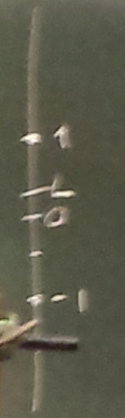
\includegraphics[scale=0.4]{img/2/1}
      \caption{Zeichnung zu 2.}
    \end{figure}    
    
    \item $a>0 \implies \lim_{n\to \infty} a^\frac{1}{n}=1$ Siehe Übung
    
    \item $\lim_{n \to \infty} n^\frac{1}{n}=1$ Siehe Übung 
    
    \item Sei $q\in \mathbb{R}, |q|<1$
    
    $\implies \lim_{n \to \infty} q^n=0$
    
    $\implies \frac{1}{|q|}>1 \implies h:=\frac{1}{|q|}-1>0$
    
    Sei $\epsilon > 0$: Aus Bernoulli: 
    
    $|q|^{-n}=(1+h)^n \geq 1+n*h> n*h>\frac{1}{\epsilon}$
    
    für $n> \frac{1}{\epsilon*h}=:k_\epsilon$
    
    $\implies |q^n-0|=|q^n|=|q|^n < \frac{1}{n*h} < \epsilon$
    
    für alle $n > \frac{1}{\epsilon*h}$
    
    \item $\forall q \in \mathbb{R}, |q|<1,p \in \mathbb{N}$
    
    $\lim_{n \to \infty} n^p*q^n=0$
    
    \textbf{Beweis} O.B.d.A $a \neq 0$
    
    $h := \frac{1}{|q|}-1$
    
    $\implies |q|^{-n} = (1-h)^n = \sum_{k=0}^n \binom{n}{k} h^k$
    
    Sei $\boxed{n>2p} > \binom{n}{p+1} h^k$
    
    $=\frac{n!}{(p+1)!(n-p-1)!} h^{p+1}$
    
    $\underbrace{n*(n-1)*\ldots*(n-p)}_{p+1 \text{ Faktoren}}*\frac{h^{p+1}}{(p+1)!}$
    
    $>\left(\frac{n}{2}\right)^{p+1} \frac{h^{p+1}}{(p+1)!}$
    
    $\implies |p|^n < \left(\frac{2}{h}\right)^{p+1} \frac{(p+1)!}{h^{p+1}}$
    
    $\implies n^p|q|^h < \frac{2^{p+1}(p+1)!}{h^{p+1}}*\frac{1}{n}$
    
    Sei $\epsilon >0$ wähle $k_\epsilon \in \mathbb{N}$,
    
    $k_\epsilon > max\left(2p,\frac{h^{p+1}}{2^{p+1}(p+1)!}*\frac{1}{\epsilon}\right)$
    
    $\implies |n^p*q^n-0|=n^p|q|^n < \epsilon \quad \forall n \geq k_\epsilon$
  \end{enumerate}
\end{example}

\textbf{Notation} Sei $n \in \mathbb{N}$, $A(n)$ Aussagen.

Wir sagen $A(n)$ ist wahr für fast alle $n$, falls $\exists k \in \mathbb{N}: A(n)$ ist wahr $\forall n \geq k$

(Oder: $A(n)$ ist wahr bis auf endlich viele $n$)

\begin{example}
  $\lim a_n = L \Longleftrightarrow \forall \epsilon > 0: |a_n-L|<\epsilon$ für fast alle $n$
  
  $\Longleftrightarrow \forall \epsilon > 0$ sind fast alle $a_n$ in einer $\epsilon$-Umgebung von $L$.
\end{example}

\subsubsection{Satz 3}

\begin{enumerate}

  \item Sei $(a_n)_n$ eine konvergente Folge, dann ist der Grenzwert eindeutig!
  
    \begin{proof}
    
      \textbf{Angenommen} $a_n \to L$ und $a_n \to R,L\neq R$
      
      \begin{figure}[!ht]
        \centering
          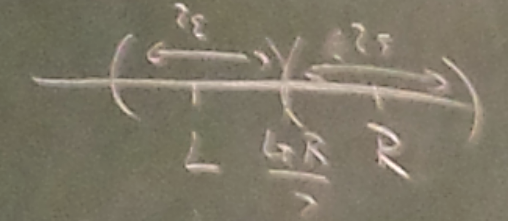
\includegraphics[scale=0.4]{img/2/2}
        \caption{Zeichnung zum Beweis}
      \end{figure}          
      
      $L<R \quad \epsilon := \frac{R-L}{2} >0$
      
      Dann gilt: $\exists k_1 \in \mathbb{N}:|a_n - L|< \epsilon \quad \forall n \geq k_1$
      
      $\exists k_2 : |a_n -R| < \epsilon \quad \forall n \geq k_2$
      
      $\implies n \geq max(k_1,k_2): a_n-L > \epsilon$ und $a_n-R < \epsilon$
      
      $\implies a_n < L+\epsilon = L+\frac{R-L}{2}=\frac{R+L}{2}$
      
      $=R-\epsilon < a_n \lightning$
    \end{proof}  
  
  \item Sei $(a_n)_n$ eine konvergente Folge, dann ist sie beschränkt, d.h. $\exists M \in [0,\infty):|a_n|\leq M \forall n \in \mathbb{N}$
  
  \begin{proof}

    Sei $\epsilon = 1 \implies \exists k_1 \in \mathbb{N}: |a_n -L| < 1$ und $n \geq k_1$
    
    $\implies |a_n| = |a_n-L+L| \leq |a_n -L|+ |L|<|L|+1$
    
    $\implies M:= max(|a_1|,|a_2|,\ldots,|a_{k_1}|,|L|+1)$
    
    $\implies |a_n| \leq M \quad \forall n \in \mathbb{N}!$
    
  \end{proof}
\end{enumerate}

\subsubsection{Lemma 4}

Sein $(a_n)_n,(b_n)_n$ Folgen

$a_n \to L, a_n-b_n \to 0$ (WORT?!? $a_n-b_n$ ist eine Nullfolge)

\begin{proof}

  Typisches $\frac{\epsilon}{2}$ Argument
  
  \begin{tabular}{rl}
    Sei $\epsilon > 0 \implies$ existiert & $k_1(\epsilon): |a_n-L|<\frac{\epsilon}{2} \quad \forall n \geq k_1(\epsilon)$ \\
    
                                      und & $k_2(\epsilon): |a_n-b_n|<\frac{\epsilon}{2} \quad \forall n \geq k_2(\epsilon)$
  \end{tabular}
  
  Setze: $k(\epsilon):=max(k_1(\epsilon),k_2(\epsilon))$
  
  $|b_n-L| = |b_n-a_n+a_n-L|$
  
  $\leq |b_n -a_n|+|a_n-L|$
  
  $<\frac{\epsilon}{2}+\frac{\epsilon}{2}=\epsilon$
  
  \begin{figure}[!ht]
    \centering
      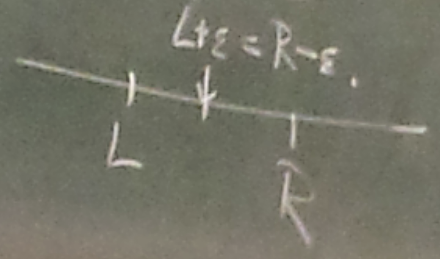
\includegraphics[scale=0.4]{img/2/3}
    \caption{Zeichnung zum Beweis}
  \end{figure}
 
\end{proof}

\subsubsection{Satz 5: Rechenregeln für Limes}

Sei $a_n\to a, b_n \to b, \lambda $ eine Zahl.

\begin{enumerate}
  \item $\lim(a_n+b_n)=a+b$
  
    $\lim(\lambda*a_n)=\lambda*a$
    
    $\lim(a_n*b_n)=a*b$
    
    und falls $b \neq 0 \implies b_1 \neq 0$ für fast alle $n$: $\lim \frac{a_n}{b_n} = \frac{a}{b}$ 
 
  \begin{proof}
    
    $\frac{\epsilon}{2}$ Angenommen.
    
    \begin{tabular}{rl}
      Sei $\epsilon > 0$ & $\exists k_1:|a_n-a|<\frac{\epsilon}{2} \quad \forall n \geq k_1$ \\
    
                         & $\exists k_2:|b_n-b|<\frac{\epsilon}{2} \quad \forall n \geq k_2$
    \end{tabular}

    $\implies$ für $n\geq k := \max(k_1,k_2)$ gilt

    $|(a_n+b_n)-(a+b)|=|a_n-a+b_n-b|$
  
    $\leq |a_n-a| + |b_n-b| < \frac{\epsilon}{2}+\frac{\epsilon}{2}= \epsilon$
  
    \textbf{Produkt:} $a_n*b_n-a*b=(a_n-a)b_n+a(b_n-b)$
  
    $=|a_n*b_n -a*b| \leq |a_n-a||b_1|+|a||b_n-b|$
    
    $b_n \to b \implies |b_n|$ ist beschränkt 
    
    d.h. $\exists 0 < M < \infty: |b_1| \leq M \quad \forall n$
    
    \begin{tabular}{rl}
      \textbf{Gegeben} $\epsilon > 0$ Wähle & $k_1: |a_n-a|<\frac{\epsilon}{2M} \quad \forall n \geq k_1$ \\
                                            & $k_2: |b_n-b|<\frac{\epsilon}{2(|a|+1)} \quad \forall n \geq k_2$
    \end{tabular}

	$\implies \forall n > \max(k_1,k_2):$


    \begin{tabular}{rl}
      $|a_nb_n-a*b|$ & $\leq |a_n-a||b_n|+|a||b_n-b|$ \\
                     & $< \frac{\epsilon}{2M}M+|a|\frac{\epsilon}{2(|a|+1)} \leq \epsilon$
    \end{tabular}
    
    \textbf{Quotient} $\frac{a_n}{b_n}=a_n*\frac{1}{b_n}$
    
    d.h. reicht zu zeigen, dass $\frac{1}{b_n} \to \frac{1}{b}$
    
    $b_n \neq 0$ für fast alle $n \quad b \neq 0$
    
    
    $\epsilon = \frac{|b|}{2} \implies |b_n-b|<\frac{|b|}{2}$ für fast alle $n$.
    
    \begin{tabular}{rl}
      $\implies |b_n| =$  & $ |b+b_n-b| \geq |b|-|b_n-b|$  \\
                      $>$ & $ |b| - \frac{|b|}{2}=\frac{|b|}{2}>0$ für fast alle $n$
    \end{tabular}    
    
    $\implies b_n \neq 0$ für fast alle $n$.
    
    $|\frac{1}{b_n}-\frac{1}{b}|=|\frac{b-b_n}{b*b_n}|=\frac{1}{|b||b_n|}|b-b_n| \stackrel{\text{ für fast alle } n}{\leq}\frac{2}{|b|^2}|b_n-b|$

    Da $b_n \to b \implies |b_n-b| < \frac{|b|^2}{2} \epsilon$ für fast alle $n$
    
    $\implies |\frac{1}{b_n}-\frac{1}{b}|\leq \frac{2}{|n|^2}|b_n-b|<\epsilon$ für fast alle $n$

  \end{proof} 
  
  \item $\lim |a_n| = |a|$
  
  \begin{proof}
    Da $||a_n|-|a|| \leq |a_n-a|$ ist er einfach 
  \end{proof}
  
  \item Aus $a_n \leq b_n$ für fast alle $n$ folgt $a \leq b$
  
  Insbesondere: $a_n \geq 0$ für fast alle $n$

  $\implies a \geq 0$
  
  \begin{proof}
  
    Kontraposition $a_n\to a,b_n \to b$
    
    Sei $a>b$
    
    \begin{figure}[!ht]
      \centering
        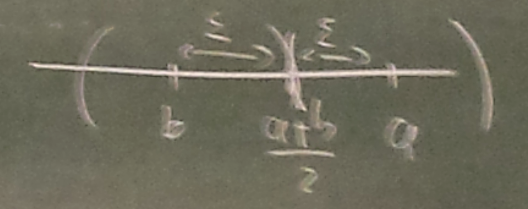
\includegraphics[scale=0.4]{img/2/4}
      \caption{Zeichnung zum Beweis}
    \end{figure}
    
    Sei $\epsilon = \frac{a-b}{2}>0$
    
    \begin{tabular}{rl}
      $\implies [a_n > a-\epsilon =$ & $ a- \frac{a-b}{2} = \frac{a+b}{2}$ \\
                                $=$ & $b+\frac{a+b}{2}=b+\epsilon>b_n]$
    \end{tabular} 
    
    für fast alle f*cking $n$.    
    
  \end{proof}
    
\end{enumerate}

\subsubsection{Satz 6} 

\begin{enumerate}
  \item Ist $(a_n)_n$ eine Nullfolge, d.h. $a_n \to 0$ und $(c_n)_n$ beschränkt $\implies (a_n*c_n)_n$ eine Nullfolge.
  
  \begin{proof}
    Es gelte $|c_n| \leq C < \infty$
    
    $b_n := a_nc_n \implies |b_n| \leq C|a_n|$
    
    d.h. 2) $\implies$ 1)    
    
  \end{proof}  
  
  \item Aus $a_n \to 0, |b_n| \leq C|a_n|$ für fast alle $n$ 
  
  ($C$ ist eine Konstante) $\implies b_n \to 0$
  
  \begin{proof}
    Sei $\epsilon > 0$ zu $\epsilon_1 := \frac{\epsilon}{C} \exists k_{\epsilon_1} : |a_n| < \epsilon_1 \forall n \geq k_{\epsilon_1}$
    
    $\implies b_n \to 0$
  \end{proof}
  
\end{enumerate}

\subsubsection{Satz 7: Sandwich Theorem}

Sei $(a_n)_n$, $(b_n)_n$ konvergente Funktionen 

mit $\lim a_n  = \lim b_n = a$ 

und $(c_n)_n*a_n \leq c_n \leq b_n$ für fast alle $n$

$\implies (c_n)_n$ konvergiert und bei $c_n=a$

\begin{proof}
  Sei $\epsilon > 0$
  
  $\exists k_1: a_n \leq c_n \leq b_n \quad \forall n \geq k_1$
 
  $\exists k_2: |a_n-a|<\epsilon \quad \forall n \geq k_2$
  
  $\exists k_3: |b_n-a|<\epsilon \quad \forall n \geq k_3$
  
  $\implies \forall n \geq \max(k_1,k_2,k_3)$

  $a-\epsilon < a_n \leq c_n \leq b_n < a+\epsilon$

  d.h. $|c_n -a| \leq \epsilon$  
  
\end{proof}

\begin{example}

  \begin{itemize}
    \item $\forall p \mathbb{N}: \lim_{n\to \infty} (n^p)^{\frac{1}{n}}=1$
    
    \begin{proof}
      \begin{itemize}
        \item $p=1:$ Übung!
        
        \item $p=2: \lim(n^2)^{\frac{1}{n}} = \lim(n^{\frac{1}{n}}*n^{\frac{1}{n}})$
        
          $= \lim_{n \to \infty} n^{\frac{1}{n}}* \lim_{n \to \infty} n^{\frac{1}{n}}$ 

	      $1*1=1$
	    \item $p \geq 2$ Induktionsbeweis
      \end{itemize}
    \end{proof}
    \item $\lim \frac{a*n+b}{c*n+a} = \frac{a}{c}$ falls $c\neq 0$
    
    \begin{proof}
      $\frac{a*n+b}{c*n+a} = \frac{a+\frac{b}{n}}{c+\frac{d}{n}} \stackrel{\text{ Quotientenregel }}{\to} \frac{a}{c}$
    \end{proof}
        
    $\lim_{n\to \infty} \frac{a*n+d}{c*n^2+d*n+f}\neq \stackrel{c \neq 0 }{0}$
    
    \begin{proof}
      $\frac{a*n+d}{c*n^2+d*n+f}= \frac{1}{n}*\frac{a+\frac{d}{n}}{c+\frac{d}{n}+\frac{f}{n^2}} \to \stackrel{c\neq 0}{0}$
    \end{proof}
  \end{itemize}

\end{example}

\subsection{Divergente Folge}
\subsubsection{Definition 8} Eine Folge $(a_n)_{n \in \mathbb{N}}$ heißt bestimmt divergent gegen $\infty$ (bzw. $-\infty$), in Zeichen, $\lim_{n\rightarrow \infty} = \infty, a_n \rightarrow \infty$ (bzw. $\lim_{n\rightarrow\infty} a_n = - \infty , a_n \rightarrow - \infty$) falls $\forall k > 0 \exists N = N(k): a_n > k \forall n \geq N$ (bzw. $a_n < -k \forall n \geq N$)\\
z.B. $a_n = n, a_n = n^2$
\subsubsection{Rechenregeln} Die regeln von S4 gelten sofern die rechten Seiten Definiert sind.\\
z.B. $a_n = n, b_n = n^2 \implies a_n + b_n \rightarrow \infty + \infty = \infty$, also $a_n - b_n \rightarrow \infty - \infty$ nicht definiert\\
$n - n^2 = (\frac{1}{n} - 1) n^2 \leq -\frac{1}{2}n^2, n\geq 2 \rightarrow \infty$\\
insb gilt:
\begin{enumerate}[1)]
\item $a_n \rightarrow \infty \implies \lambda a_n \rightarrow \infty$ für $\lambda > 0, \lambda a_n \rightarrow - \infty, \lambda < 0$
\item $a_n \rightarrow \infty \rightarrow \frac{1}{a_n} \rightarrow 0$ und falls $a_n > 0$ für fast alle n, dann gilt auch Umkehrung
\item $a_n \rightarrow \infty, b_n \rightarrow b \in \mathbb{R} \implies a_n + b_n \rightarrow \infty$
\item $a_n \rightarrow \infty, b_n \rightarrow b > 0$ (oder $b_n \rightarrow \infty$) $\implies a_n * b_n \rightarrow \infty$
\end{enumerate}
\begin{proof}
\begin{itemize}
\item 1) - 3): Scharf hinschauen
\item 4) $b_n \rightarrow b > 0 \implies b_n \geq \frac{1}{2} b$ für fast alle n, $\implies a_n * b_n > \frac{1}{2}b*a_n$ für fast alle n.\\zu $k > 0$, wähle $N(k): a_n > \frac{2}{b}k \forall n\geq N(k)$\\$\implies a_n * b_n > \frac{b}{2} * \frac{2}{b} k = k$ für fast alle n
\end{itemize}
\end{proof}
\subsection{Monotone Folgen}
\subsubsection{Definition 9} Eine Folge $(a_n)_n$ reeller Zahlen heißt
\begin{enumerate}[1)]
\item wachsend, falls $a_n \leq a_{n+1} \forall n \in \mathbb{N}$
\item fallend, falls $a_n \geq a_{n+1} \forall n \in \mathbb{N}$
\item monoton, falls sie wachsend oder fallend ist.
\end{enumerate}
\subsubsection{Satz 10 (Monotone Konvergenz)} Jede beschränkte monotone Folge ist konvergen! Insb:
\begin{enumerate}[1)]
\item $(a_n)_n$ wachsend (beschränkt) $\implies \lim_{n\rightarrow\infty} a_n = \sup_{n\in\mathbb{N}}a_n$
\item $(a_n)_n$ fallend (beschränkt) $\implies \lim_{n\rightarrow \infty} a_n = \inf_{n\in\mathbb{N}}a_n$
\end{enumerate}
\begin{proof}
\begin{enumerate}[1)]
\item Sei $a:=\sup a_n = \sup \{a_n: n\in\mathbb{N}\}\in\mathbb{R}$ wegen Vollständigkeitsaxiom\\
Sei $a>0$. Nach Definition von Supremum $\exists k_\epsilon \in \mathbb{N}$\\
$\alpha - \epsilon < a_{k_\epsilon} \leq a_{\k-{\epsilon + 1}} \leq ... \leq a_n \leq \alpha \forall n \leq k_\epsilon$
\item Wende 1) auf $b_n = -a_n a_n$
\end{enumerate}
\end{proof}
\subsubsection{Korollar 11} Sei $(b_n)_n$ Folge mit $\frac{|b{n+1}|}{|b_n|} \rightarrow x$ für $o \leq x < 1 \implies \lim b_n = 0$\\insb. $\lim q^n = 0, |q|<1$

\begin{proof}
Z.z. $|b_n| \rightarrow 0$ d.h. O.B.d.A. $b_n > 0$. Da $\frac{b_{n+1}}{b_n} \rightarrow x$ für $0 \leq x < 1$\\
Wähle $s = 1 -x > 0 \implies \exists N$\\
$\frac{b_{n+1}}{b_n} < x + \epsilon = 1 \forall n \geq N$\\
$\implies b_{n+1} < b_n \forall n \geq N$\\
$\implies L = \lim_{n \rightarrow \infty} b_n$ existiert und $L \geq 0$. Wollen $L = 0$\\
\paragraph{Angenommen:} $L>0$\\$\implies [x = \lim \frac{b_{n+1}}{b_n} \underbrace{=}_{\text{Quotientenmenge}} \frac{\lim b_{n+1}}{\lim b_n} = \frac{L}{L} = 1] \lightning$ d.h. $L = 0$!
\end{proof}
\subsubsection{Korollar 12 (Rekursive Berechnung von $\sqrt{a}$} Sei $a > 0, x_0 > 0$. Definiere $(x_n)_{n\in\mathbb{N}}, x_{n+1} := \frac{1}{2} (x_n+ \frac{a}{x_n}) | n\in\mathbb{N}$. Dann konvergiert $x_n, \lim x_n = \sqrt{a}, x_n > 0 \forall n$

\begin{proof}
Per Induktion zeigt man $x_n > 0 \forall n$
\end{proof}
\begin{enumerate}[\text{Fakt }1:]
\item $x_n \geq \sqrt{a} \forall n > 1,$ da $x_{n+1}^2 -a = \frac{1}{4}(x_n - \frac{a}{x_n})^2 - a$\\
$= \frac{1}{4}(x_n^2 - 2a + \frac{a^2}{x_n^2}  4a)$\\
$= \frac{1}{4}(x_n-\frac{a}{x_n})^2 \geq 0$
\item Für $n \geq 1$ ist $(x_n)_n$ fallend, \\da $x_n - x_{n+1} = x_n - \frac{1}{2} (x_n + \frac{a}{x_n}) = \frac{1}{2}(x_n - \frac{a}{x_n})$\\
$=\underbrace{\frac{1}{2x_n}}_{\geq 0} \underbrace{(x_n^2 -a}_{\geq 0} \geq 0$ wegen Fakt 1) \\
$\implies \lim_{n \rightarrow \infty} x_n = x$ existiert $\geq \sqrt{a}$\\
$\implies x = \lim x_{n+1} = \frac{1}{2} \lim (x_n + \frac{a}{x_n} = \frac{1}{2} (x + \frac{a}{x})$\\
$\implies x^2 = a$, da $x > 0 \implies x = \sqrt{a}$

\begin{proof}

$f_n := x_n - \sqrt{a} \implies f_{n+1} = x_{n+1} - \sqrt{a} = \frac{1}{2}(x_n + \frac{a}{x_n}) - \sqrt{a}$\\
$= \frac{1}{2x_n}(x_n^2 -a) - \sqrt{a} = \frac{1}{2x_n}(x_n - \sqrt{a})^2 = \frac{f_n^2}{2x_n} \leq \frac{1}{2\sqrt{a}} f_n^2$, $n\geq 1$\\
quadratische Konvergenz
\end{proof}
\end{enumerate}

\subsubsection{Korollar 13}
$e := \lim_{n \rightarrow \infty} (1 + \frac{1}{n})^n$ existiert und $2 + \frac{1}{3} < e \leq \frac{6^7}{2n} < 2,78167$

\begin{proof}
$$a_n = (1 + \frac{1}{n})^n \implies a_n\text{ ist wachsend da } n\geq 2$$
$$\frac{a_n}{a_{n-1}} = \frac{(1+\frac{1}{n})^n}{(1+\frac{1}{n-1})^{n-1}} = \frac{(\frac{n+1}{n})^n}{(\frac{n}{n-1})^{n-1}}$$
$$= \frac{n}{n-1} * (\frac{(n+1)(n-1)}{n^2})^n = \frac{n}{n-1} (\frac{n^2 - 1}{n^2})^n$$
$$= \frac{n}{n-1} (1-\frac{1}{n^2})^n \underbrace{>}_{\text{Bernoulli}} \frac{n}{n-1} (1 - n * \frac{1}{n^2}) = 1$$
Monotone Konvergenz $\implies a_n$ konvergiert, wenn es nach oben beschränkt ist.
$$a_n = (1 - \frac{1}{n})^n = \sum_{k = 0}^n \binom{n}{k} (\frac{1}{n})^k = \sum_{k=0}^n \frac{n!}{k!(n-k)!} * \frac{1}{n^k}$$
$$= \sum_{k =0}^n \frac{1}{k!} \prod_{l=0}^k \frac{n-l}{n} \leq \sum_{k=0}^n \frac{1}{k!}$$
Induktion $=: k! \geq 2^k$ für $k\geq 4$\\
$$\implies n \geq k: a_n \leq |1| + \frac{1}{2} +  \frac{1}{2k} + \sum_{k = 4}^n (\frac{1}{2})^k$$
$$= \frac{16}{6} + \frac{1}{24} \sum_{l = 0}^{n-4} (\frac{1}{2})^l = \frac{16}{6} + \frac{1}{2^4} \underbrace{(\frac{1-(\frac{1}{2})^{n-k}}{1-\frac{1}{2}})}_{\leq 2}$$
$$\leq \frac{16}{6} + \frac{1}{8} = \frac{67}{24} \implies e \leq \frac{67}{24}$$
$$e \geq a_n \forall n, n = 3$$
$$=(1 + \frac{1}{2})^k, e \geq a_3 = 2 + \frac{10}{27} > 2 + \frac{1}{3}$$
\end{proof}
\subsection{Teilfolgen und Häufungswerte}
\subsubsection{Definition 14: (Teilfolgen, Umordnung)} $(a_n)_n$ Folge $a = (a_n)_{n+1}: \mathbb{N} \rightarrow \mathbb{R}$\\
$\phi : \mathbb{N} \rightarrow \mathbb{N}$ bijektiv\\
$\implies b:= a = \phi$, d.h. $b = (b_l)_{l\in\mathbb{N}}$, $b_l := a_{\phi (l)}$\\
Umordnung von $(a_n)_n$\\
Wir nenn $\sigma : \mathbb{N} \rightarrow \mathbb{N}$ eine Verdünnung falls $\sigma$ strikt monoton steigend ist, d.h. $\sigma (n) < \sigma (n+1) \forall n$. Dann ist $(b_l)_l$ definiert durch $b_l := a_{\sigma (l)}$ eine Teilmenge von $(an)_n$
\paragraph{Bemerkung:}
\begin{enumerate}[1)]
\item Für jede Verdünnung $\sigma$ gilt $\sigma (n) \geq n \forall n \in \mathbb{N}$ (Warum?)
\item $(a_n)_n := (\frac{1}{n})_n$, $(\frac{1}{2l})_l$, $(\frac{1}{l^2})_l$ sind Teilfolgen von $(a_n)_n$\\
$\sigma(n) = 2n$, $b_{\sigma(l)} = a_{2l} = \frac{1}{2l}$\\
$\sigma(n) = n^2$, $b_n = a_{\sigma(n)} = a_n^2 = \frac{1}{n^2}$\\
$(\frac{1}{2}, 1, \frac{1}{4}, \frac{1}{3}, \ldots$ ist eine Umordnung von $(1, \frac{1}{2}, \frac{1}{3}, \frac{1}{4}, \ldots)$
\end{enumerate}
\subsubsection{Lemma 15} Jede Umordnung und jede Teilmenge einer konvergierten Folge konvergiert auf dem selben Grenzwert. Und dasselbe gilt, wenn mman aus endlichviele Werte vpn $a_n$ abändert.

\begin{proof}
Für Umordnung nachrechnen.\\
Sei $b_n = a_{\sigma(n)}$ Teilfolgen von $(a_n)_n$\\
$a_n \rightarrow L: \forall \epsilon > 0 \exists k_\epsilon: |a_n - L| < \epsilon \forall n \geq k_\epsilon$\\
Da $\sigma(n) \geq n \forall n \in \mathbb{N}$ gilt auch $\forall n \geq k_\epsilon$\\
$|b_n - L| = |a_{\sigma(n)} - L| < \epsilon$
\end{proof}
\subsubsection{Definition 16 Häufungswert}
Sei $(a_n)_n$ eine Folge, $a\in\mathbb{R}$ ist ein Häufungswert von $(a_n)_n$, falls $\forall \epsilon > 0$ gibt unendlich viele $n\in\mathbb{N}$ mit $|a_n - a| < \epsilon$
\paragraph{Beispiel} $a_n = \frac{1}{2}$ hat HW 0\\
$a_n = (-1)^n$ hat HW 1 und -1\\
$a_n = (-1)^n + \frac{1}{n}$ hat HW 1 und -1\\
$H((a_n)_n) = $ Menge der HW von $(a_n)_n = \{ a\in\mathbb{R}$, $a$ ist HW von $(a_n)_n\}$
\paragraph{Bemerkung}
\begin{enumerate}[1)]
\item Für eine beschränkte Folge $(a_n)_n$ gilt: $$a_n \rightarrow a \Leftrightarrow H((a_n)_n) = \{a\}$$
\item $(n)_{n\in\mathbb{N}}$ hat keine HW!
\end{enumerate}
\subsubsection{Satz 17 (Bolzano - Weierstraß für Folgen)} Jede beschränkte Folge hat mindestens einen HW
\begin{proof}
Sei $(a_n)_n$ beschränkt, z.B. $c \leq a_n \leq d \forall n$\\
$G := \{ x\in\mathbb{R}: a > x$ für höchstens endlich vielen$\}$\\
$=\{x\in\mathbb{R}: a_n \leq x$ für fast alle n$\}$
\begin{enumerate}[\text{Fakt }1)]
\item $G \neq \emptyset$, da $d \in G$
\item $G$ ist nach unten beschränkt, denn $x \notin G$, falls $x < c \implies \alpha := \inf G \in \mathbb{R}$\\
\paragraph{Behauptung} $a < H((a_n)_n)$\\
Dann sei $\epsilon > 0 \implies$ nach Definition von Infimum $\alpha + \epsilon \in G$ und $\alpha - \epsilon \notin G \implies$ all $a_n < \alpha + \epsilon$ udn unendlich viele $a-n > \alpha - \epsilon$\\
$\implies$ es gibt unendlich viele $n: |a_n - \alpha| < \epsilon \implies e \text{ ist HW}$
\end{enumerate}
\end{proof}
\subsubsection{Lemma 18} $(a_n)_n Folge$\\
$a \in H((a_n)_n) \Leftrightarrow \exists$ Teilfolge von $(a_n)_n$ die gegen a konvergiert.
\end{document}